\documentclass[tikz,convert={density=150,size=600,outext=.png}]{standalone}
\usetikzlibrary{shapes, calc, arrows, fit, positioning, decorations, patterns, decorations.pathreplacing, chains, snakes}

\begin{document}
  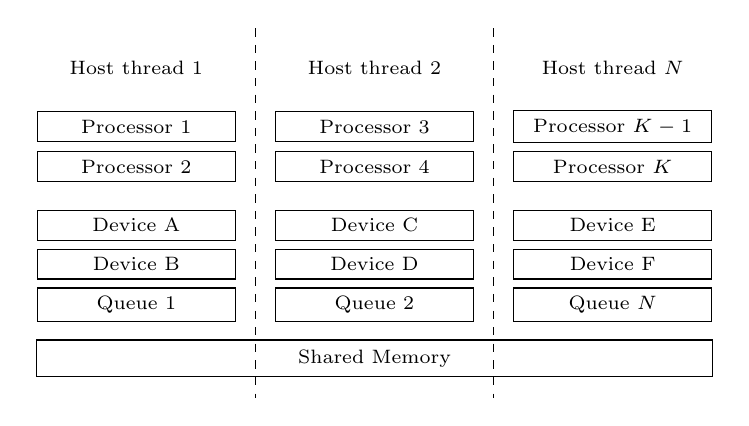
\begin{tikzpicture}[>=latex, font=\scriptsize]
    \node[matrix, column sep={0.5cm}, row sep={0.1cm},
      nodes={text width = 2.3cm, align=center, inner sep=3pt}] (separate)
    {
        \node (t1) {Host thread 1}; & \node (t2) {Host thread 2}; & \node (t3) {Host thread $N$}; \\[0.25cm]
        \node[draw] {Processor 1};  & \node[draw] {Processor 3}; & \node[draw] {Processor $K-1$}; \\
        \node[draw] {Processor 2};  & \node[draw] {Processor 4}; & \node[draw] {Processor $K$}; \\[0.25cm]
        \node[draw] {Device A};  & \node[draw] {Device C}; & \node[draw] {Device E}; \\
        \node[draw] {Device B};  & \node[draw] {Device D}; & \node[draw] {Device F}; \\
        \node[draw] {Queue 1};  & \node[draw] {Queue 2}; & \node[draw] {Queue $N$}; \\[0.25cm]
        \node[] (z1) {};  & \node[inner ysep=0pt] (z2) {Shared Memory}; & \node[] (z3) {}; \\
    };

    \node[draw, inner xsep=0pt, fit=(z1) (z2) (z3)] {};

    \draw[dashed] ([yshift=0.5cm] barycentric cs:t1=0.5,t2=0.5) -- ([yshift=-0.5cm] barycentric cs:z1=0.5,z2=0.5);
    \draw[dashed] ([yshift=0.5cm] barycentric cs:t2=0.5,t3=0.5) -- ([yshift=-0.5cm] barycentric cs:z2=0.5,z3=0.5);
  \end{tikzpicture}
\end{document}
